\documentclass[conference]{IEEEtran}
\usepackage[utf8]{inputenc}
\usepackage{times}
\usepackage{epsfig}
\usepackage{graphicx}
\usepackage{amsmath}
\usepackage{amssymb}
\usepackage{mathrsfs}
\usepackage{mwe}
\usepackage{float}
\usepackage{caption}
\usepackage{subcaption}
\usepackage{makecell}
\usepackage{indentfirst}
\usepackage{algorithmic}
\usepackage{algorithm}
\usepackage{gensymb}

\title{Team 02 EECS 467 Report}
\author{Christopher Nguyen,  Kun Huang, Zhihao Ruan}

\begin{document}

\maketitle
\begin{abstract}
In this report, we discuss about the four different control algorithms we implemented for driving the Mbot. We first implemented a closed-loop velocity to control the angular speed of the wheels and we tuned the PID for three different configurations: over-damped, under-damped and critically-damped. Next, we implemented a open-loop controller which drives the Mbot for a set amount of time and didn't use feedback from the odometry to minimize any errors. We improved on this by implementing a closed-loop controller to minimize the error between Mbot's odometry and the desire pose. Finally, we implemented another closed-loop controller but we calculate the odometry by using a lidar instead of encoders. This provided more accurate updates to the Mbot's odometry and thus a more accurate driving in the real world.
\end{abstract}

\section{Results}
\subsection{Closed-Loop Velocity Control}
We first tuned a closed-loop velocity controller for each of the wheels. These controllers will be used in the later tasks to set the velocities determined from other controllers. The PIDs were the same for both controllers and the set point was set to 7m/s. We tuned the PIDs to achieve three different configurations: overdamped, underdamped and critically damped.
\[ Overdamped: k_p=0.4, k_i=2, k_d=0 \]\\
\begin{tabular}{cc}
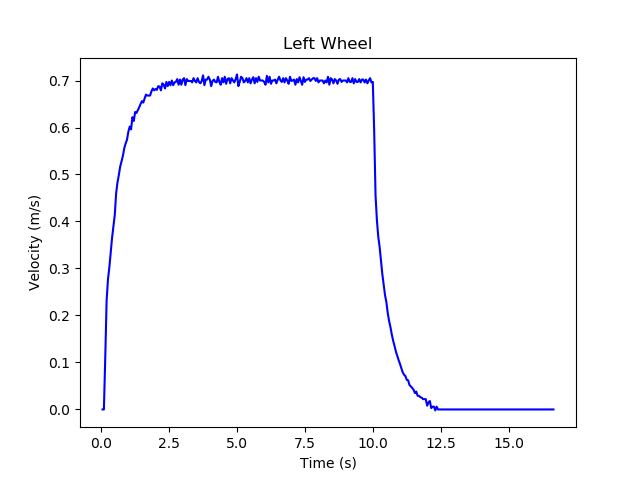
\includegraphics[width=0.45\linewidth]{step_0_4_2_0_left.png} & 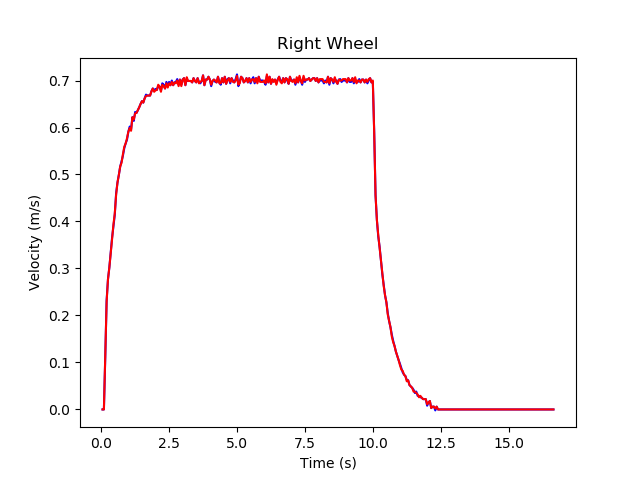
\includegraphics[width=0.45\linewidth]{step_0_4_2_0_right.png} \\
Left & Right \\[6pt]
\end{tabular}

\[ Underdamped: k_p=0.4, k_i=20, k_d=0 \]
\begin{tabular}{cc}
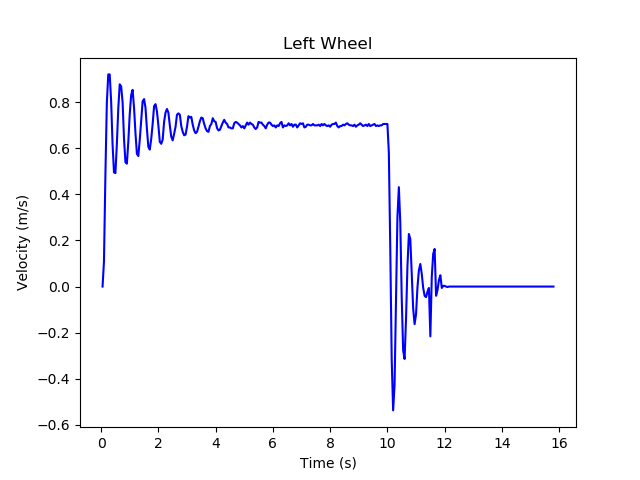
\includegraphics[width=0.45\linewidth]{step_0_4_20_0_left.png} &   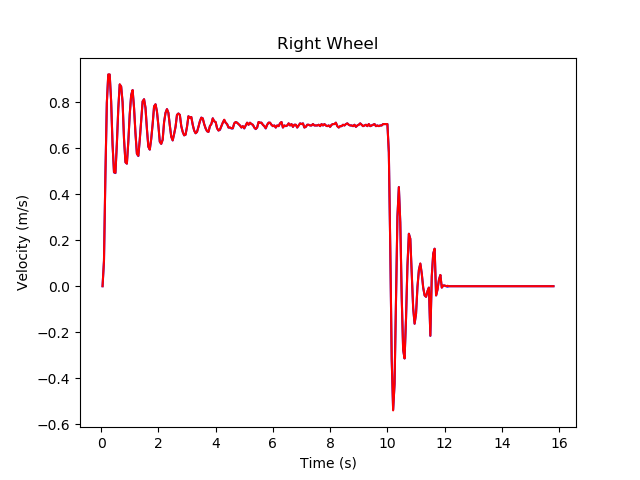
\includegraphics[width=0.45\linewidth]{step_0_4_20_0_right.png} \\
Left & Right \\[6pt]
\end{tabular}
\[ Critically-damped: k_p=0.4, k_i=6, k_d=0 \]
\begin{tabular}{cc}
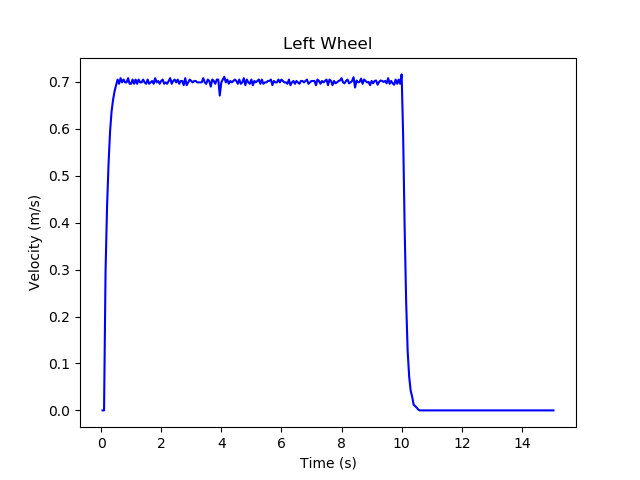
\includegraphics[width=0.45\linewidth]{step_0_4_6_0_left.png} &   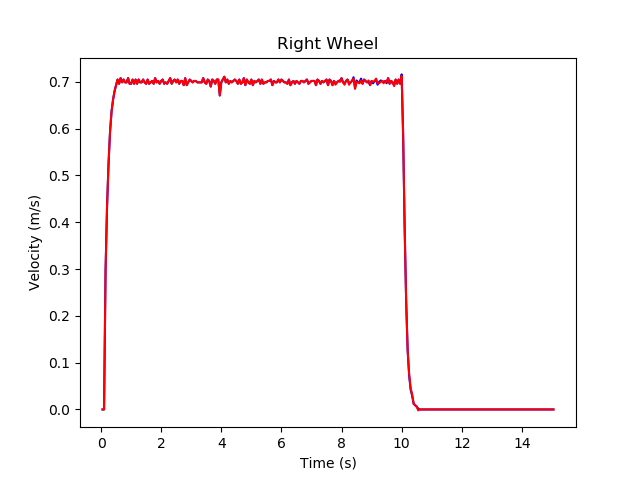
\includegraphics[width=0.45\linewidth]{step_0_4_6_0_right.png} \\
Left & Right \\[6pt]
\end{tabular}
% \begin{figure}[!htb]
% \begin{tabular}{cc}
%   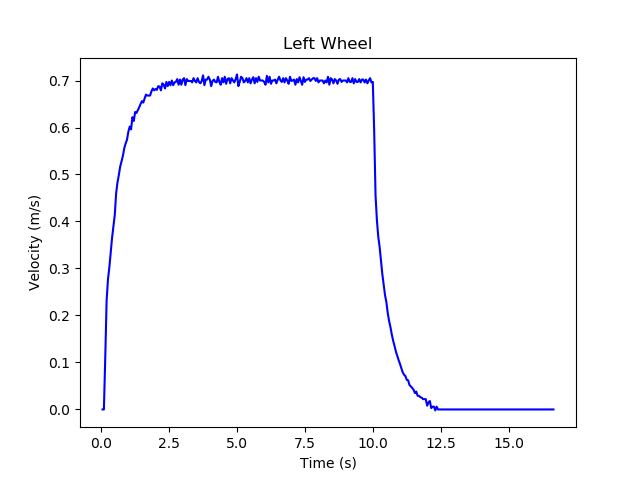
\includegraphics[width=0.45\linewidth]{step_0_4_2_0_left.png} &   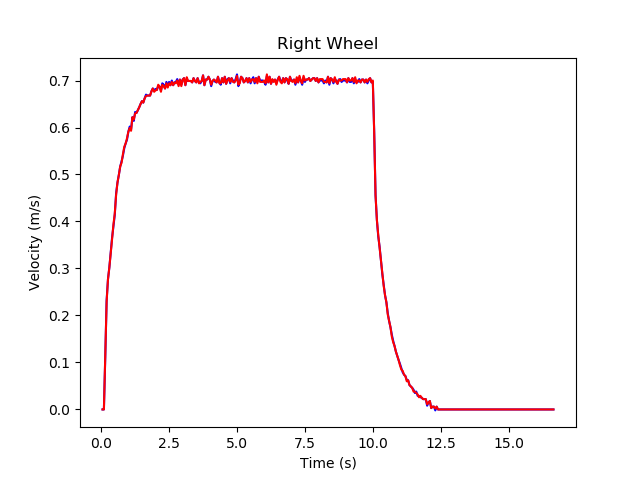
\includegraphics[width=0.45\linewidth]{step_0_4_2_0_right.png} \\
% Left wheel overdamped & Right wheel overdamped \\[6pt]
% 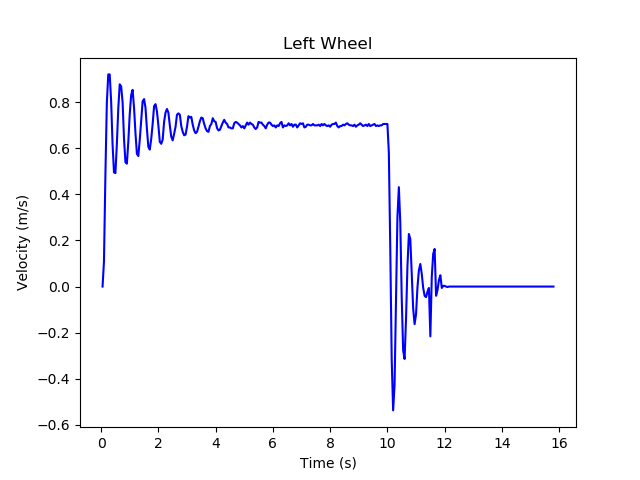
\includegraphics[width=0.45\linewidth]{step_0_4_20_0_left.png} &   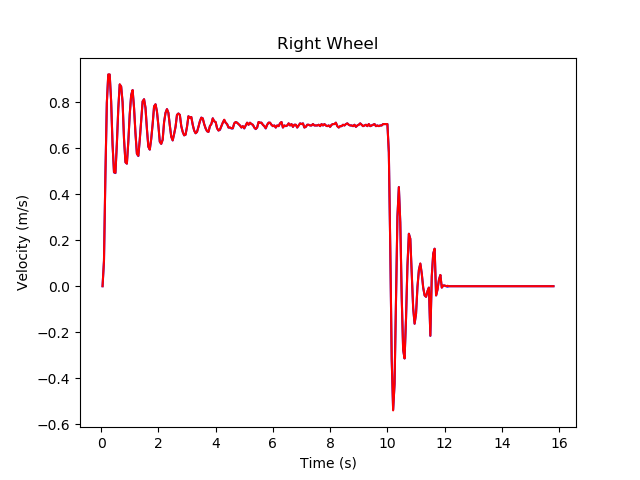
\includegraphics[width=0.45\linewidth]{step_0_4_20_0_right.png} \\
% Left wheel underdamped & Right wheel underdamped \\[6pt]
%  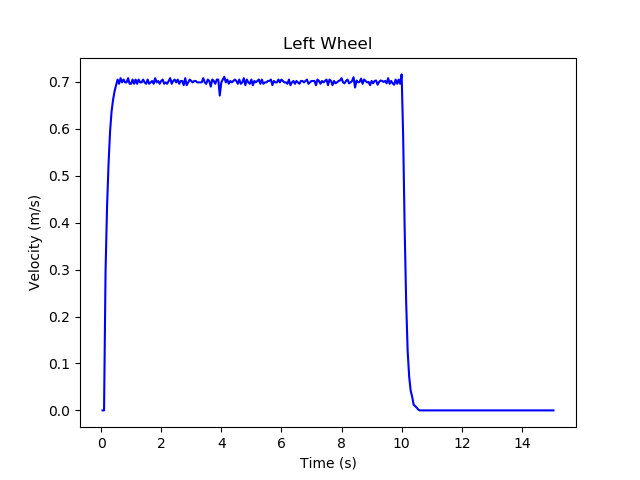
\includegraphics[width=0.45\linewidth]{step_0_4_6_0_left.png} &   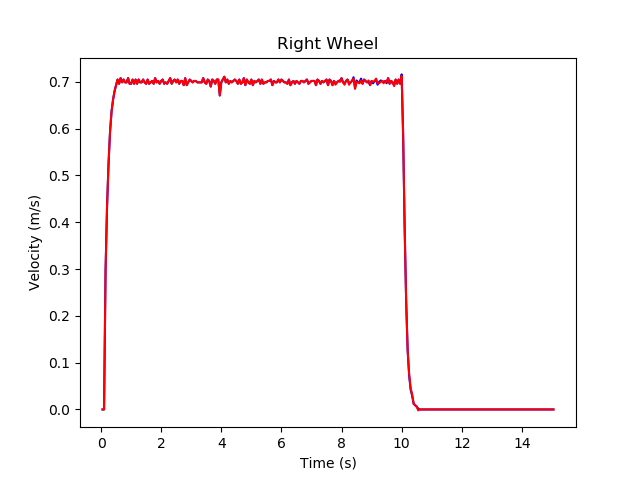
\includegraphics[width=0.45\linewidth]{step_0_4_6_0_right.png} \\
% Left wheel critically damped & Right wheel critically damped \\[6pt]
% \end{tabular}
% \caption{Velocity over time graphs for left and right wheel velocity controllers}
% \end{figure}
\subsection{Open-Loop Control}
This is a simple control algorithm which doesn't consider the robot's position and just applies a constant velocity for a predetermined amount of time. We implemented this control by utilizing the velocity controller from the previous task to apply a constant velocity to the wheels. The algorithm to drive the Mbot in a square is described below. The time to apply the velocity was calculated with $t=\frac{distance}{velocity}$, and then later tweaked with experience.
\begin{algorithm}[H]
\caption{Open Loop Control}
\begin{algorithmic}[0]
\FOR {$i = 0$ to 3}
    \FOR {$j = 0$ to 4}
        \STATE $\text{mb\_motor\_msg.ang\_v = 0.0}$\\
        \STATE $\text{mb\_motor\_msg.trans\_v = 0.2}$\\
        \STATE $\text{rc\_nanosleep(1e9)}$\\
        \STATE $\text{mb\_motor\_msg.ang\_v = -(PI * 0.25)}$\\
        \STATE $\text{mb\_motor\_msg.trans\_v = 0.0}$\\
        \STATE $\text{rc\_nanosleep(1e9)}$\\
    \ENDFOR
\ENDFOR
\end{algorithmic}
\end{algorithm}
This algorithm was not very accurate in driving. The Mbot would always drift off course and could not correct itself, resulting in the graph shown in figure 1.
\begin{figure}[H]
    \centering
    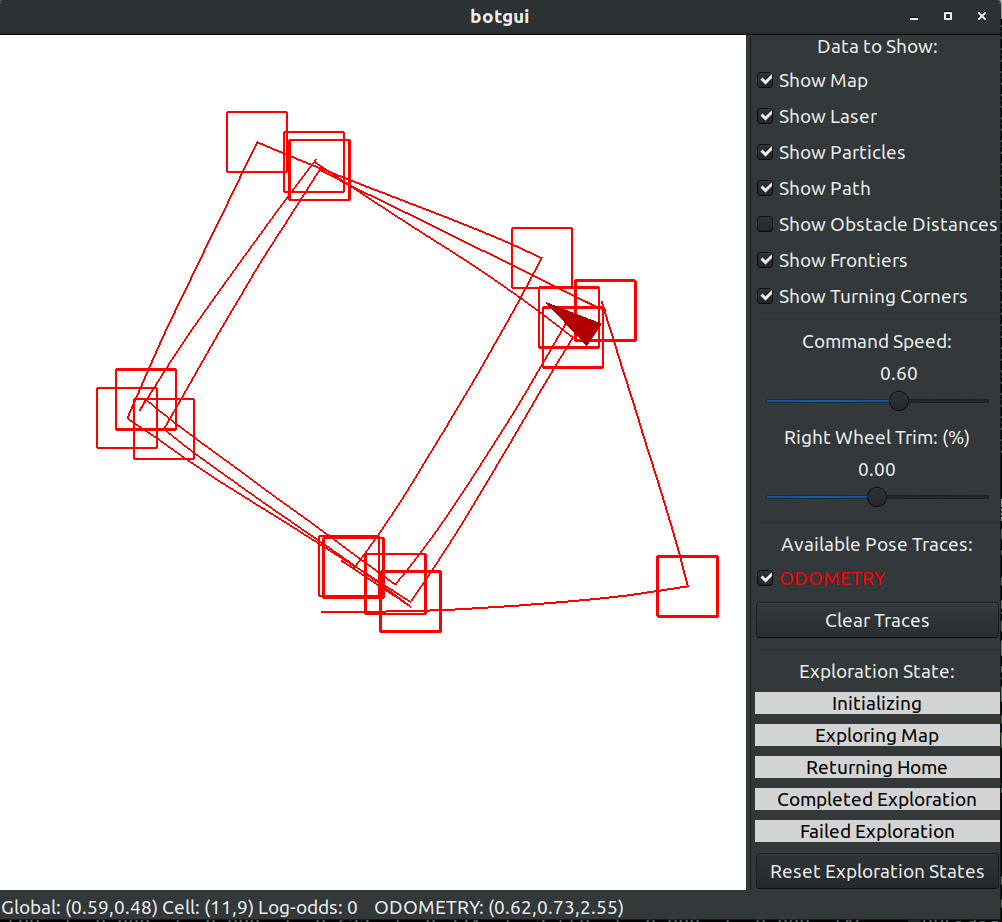
\includegraphics[width=\linewidth]{task4_corners.png}
    \caption{Driving in a square with a open-loop control algorithm}
    \label{fig:Captured Mbot's odometry when driving in a square with closed-loop controllers}
\end{figure}

\subsection{Closed Loop Control with Odometry}
We improve our driving by next implementing a closed loop control with odometry. We computed the odometry by first computing the forward and angular motion. These are computed as the following:
\[ds = \frac{enc_{left} + enc_{right}}{2} \times \frac{2 \pi R}{48 \times 34.014}\]
\[d\theta = \frac{enc_{right} - enc_{left}}{B} \times \frac{2 \pi R}{48 \times 34.014}\]
where $R = 0.04$ and $B = 0.21$. Once we get the change in motion, we use them to offset Mbot's odometry as such:
\[odo_{x} = odo_{x} + ds \times \cos(odo_{theta})\]
\[odo_{y} = odo_{y} + ds \times \sin(odo_{theta})\]
\[odo_{theta} = odo_{theta} + d\theta\]
We use the motion changes to calculate the instantaneous translational and angular velocities at that timestamp.
\[\nu_{t} = ds / DT \]
\[\omega_{t} = d\theta / DT \]
where $DT$ is the inverse of the sample rate which we read encoder counts. With the computed odometry, we use two seperate closed-loop controller. One controller outputs the translational velocities and the error it tries to minimize is the euclidean distance between Mbot's current odometry and the setpoint position. The second controllers determines the angular velocities and minimizes the difference between Mbot's theta and the setpoint theta. We use the velocity controller from Task III to set both the translational and angular velocities.\\
These two controllers significantly made Mbot's driving a lot more accurate. As shown in figure 2, the graph shows a near perfect square and display the corrections that the Mbot makes whenever it drifts off course, unlike the driving captured in figure 1.
\begin{figure}[htp]
    \centering
    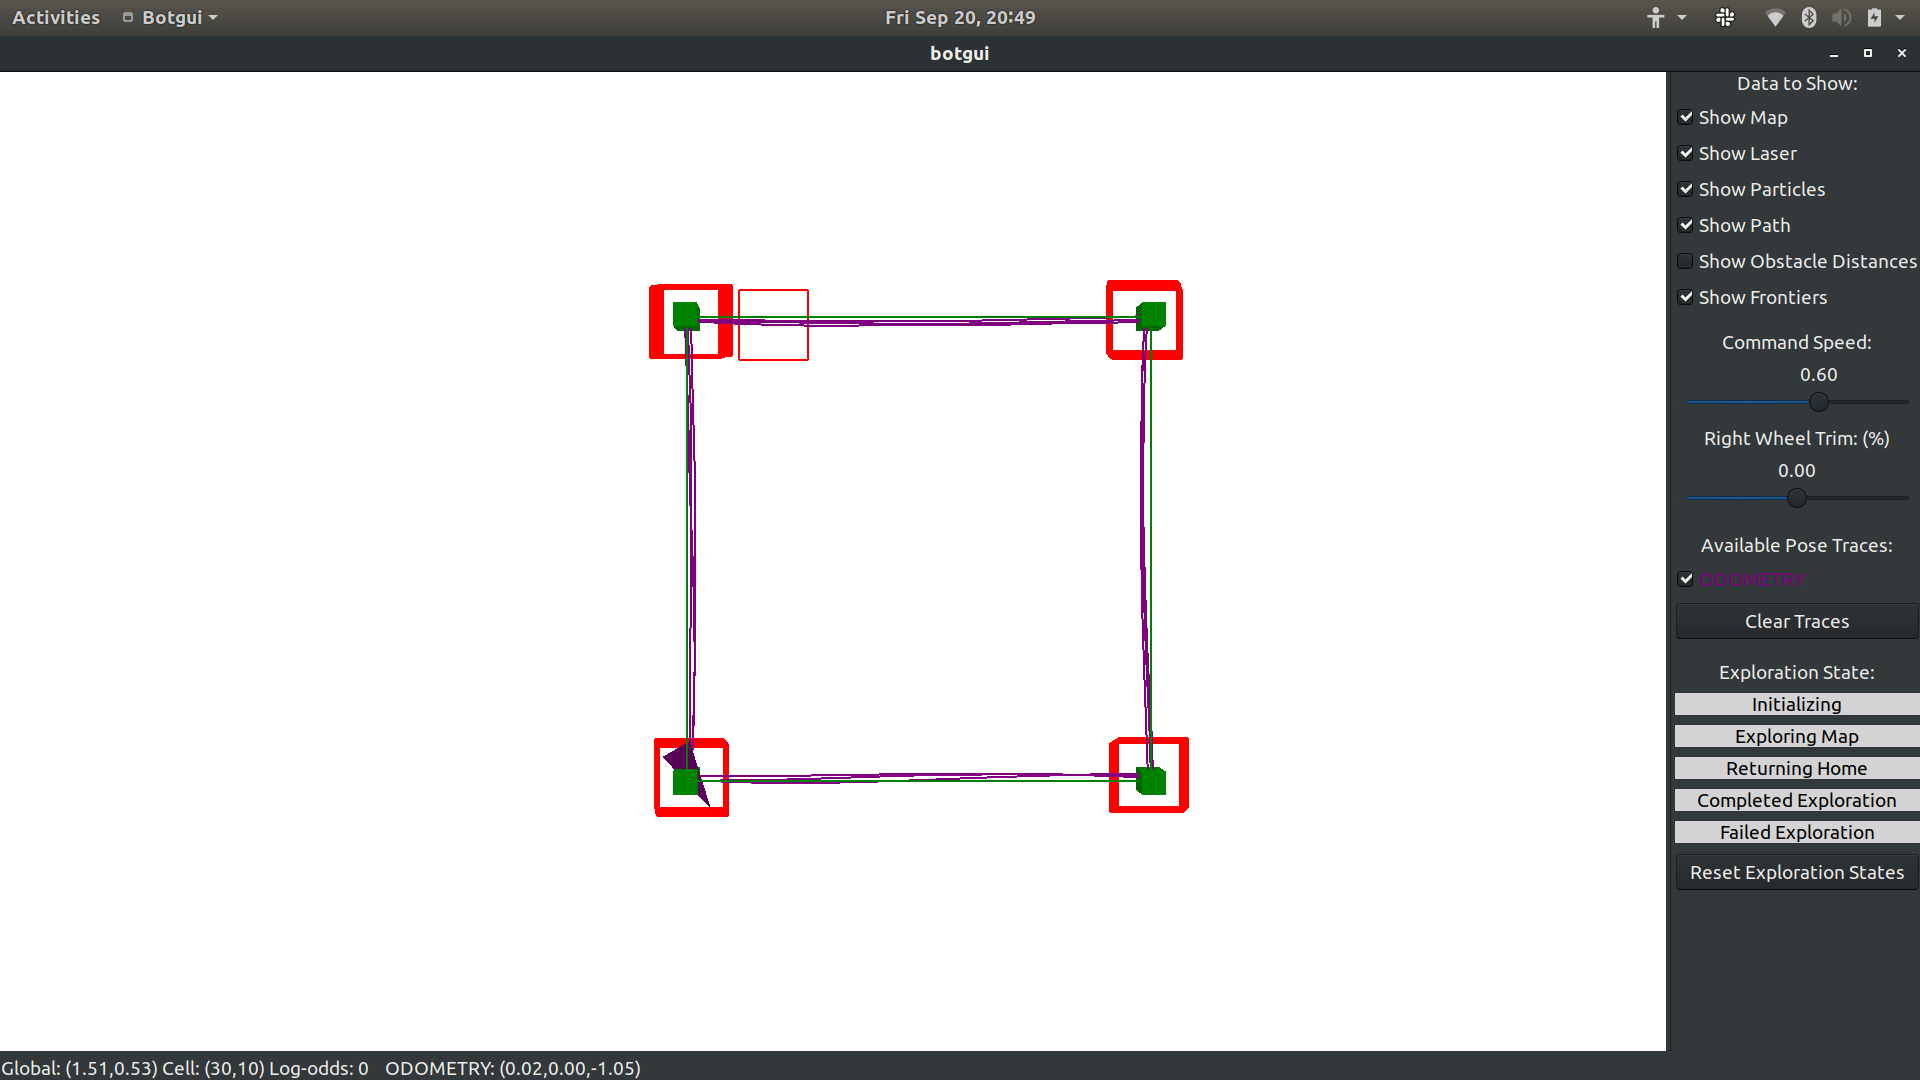
\includegraphics[width=\linewidth]{odometry_square.png}
    \caption{Captured Mbot's odometry when driving in a square with closed-loop controllers}
    \label{fig:Captured Mbot's odometry when driving in a square with closed-loop controllers}
\end{figure}


\subsection{Closed Loop Control with Laser Scans}

\begin{algorithm}[H]
\caption{Closed-loop Laser-based Controller}
\begin{algorithmic}[0]
\renewcommand{\algorithmicrequire}{\textbf{Input:}}
\renewcommand{\algorithmicensure}{\textbf{Output:}}
\REQUIRE Distance to Walls $d$, angle between robot and right wall $\theta_{rightwall}$ (counter clock-wise)
\ENSURE  Command of forward velocity and angular velocity\\
\textit{Initialisation}:
    \STATE State = DRIVE
    \STATE $\text{DESIRED\_DIST} = 0.5$
\\ \textit{LOOP Process}:
    \IF {State == TURN}
        \STATE $v = 0$
        \IF{$ d_{backwall} < \text{DESIRED\_DIST} + 0.1$\\ $\&\&\ d_{frontwall} < 2 - \text{DESIRED\_DIST} - 0.1$}
            \STATE $\omega = 0$
            \STATE State = DRIVE
        \ELSE 
            \STATE $\omega = \text{const\_turn}$
        \ENDIF
    \ELSIF{State == DRIVE}
        \IF{$d_{frontwall} < \text{DESIRED\_DIST} + 0.1$}
            \STATE $\omega = 0$
            \STATE $v = 0$
            \STATE State = TURN
        \ELSE 
            \STATE $v = \min(1.2 \times d_{frontwall} + 0.05, 0.1)$ 
            \STATE $\omega = -K_1 \times \theta_{rightwall} - K_2 / v \times (d_{rightwall} - \text{DESIRED\_DIST})$ 
        \ENDIF
    \ENDIF
\RETURN {$v$ and $\omega$}
\end{algorithmic}
\end{algorithm}


\begin{algorithm}[H]
\caption{Distance to Walls (Right Wall)}
\begin{algorithmic}[0]
\renewcommand{\algorithmicrequire}{\textbf{Input:}}
\renewcommand{\algorithmicensure}{\textbf{Output:}}
\REQUIRE Lidar data
\ENSURE  Distance to right wall $d$, angle between robot and right wall $\theta_{rightwall}$ (counter clock-wise)\\
\textit{Initialisation}:
    \STATE $d=\inf$
    \STATE $\theta_d$
    \STATE $\text{USABLE\_DATA} = 0.2$\\
\textit{LOOP Process}:
    \FOR{$ray$ in $num\_of\_rays$}
        \IF{$ray.theta \in (75^{\circ}, 105^{\circ})$ }
            \IF{$ray.range > \text{USABLE\_DATA}$}
                \IF{$ray.range < d$}
                    \STATE $d = ray.range$
                    \STATE $\theta_d = ray.theta$
                \ENDIF
            \ENDIF
        \ENDIF
    \ENDFOR
\RETURN {$d$ and $\theta_d$}
\end{algorithmic}
\end{algorithm}

\begin{figure}[H]
\centering
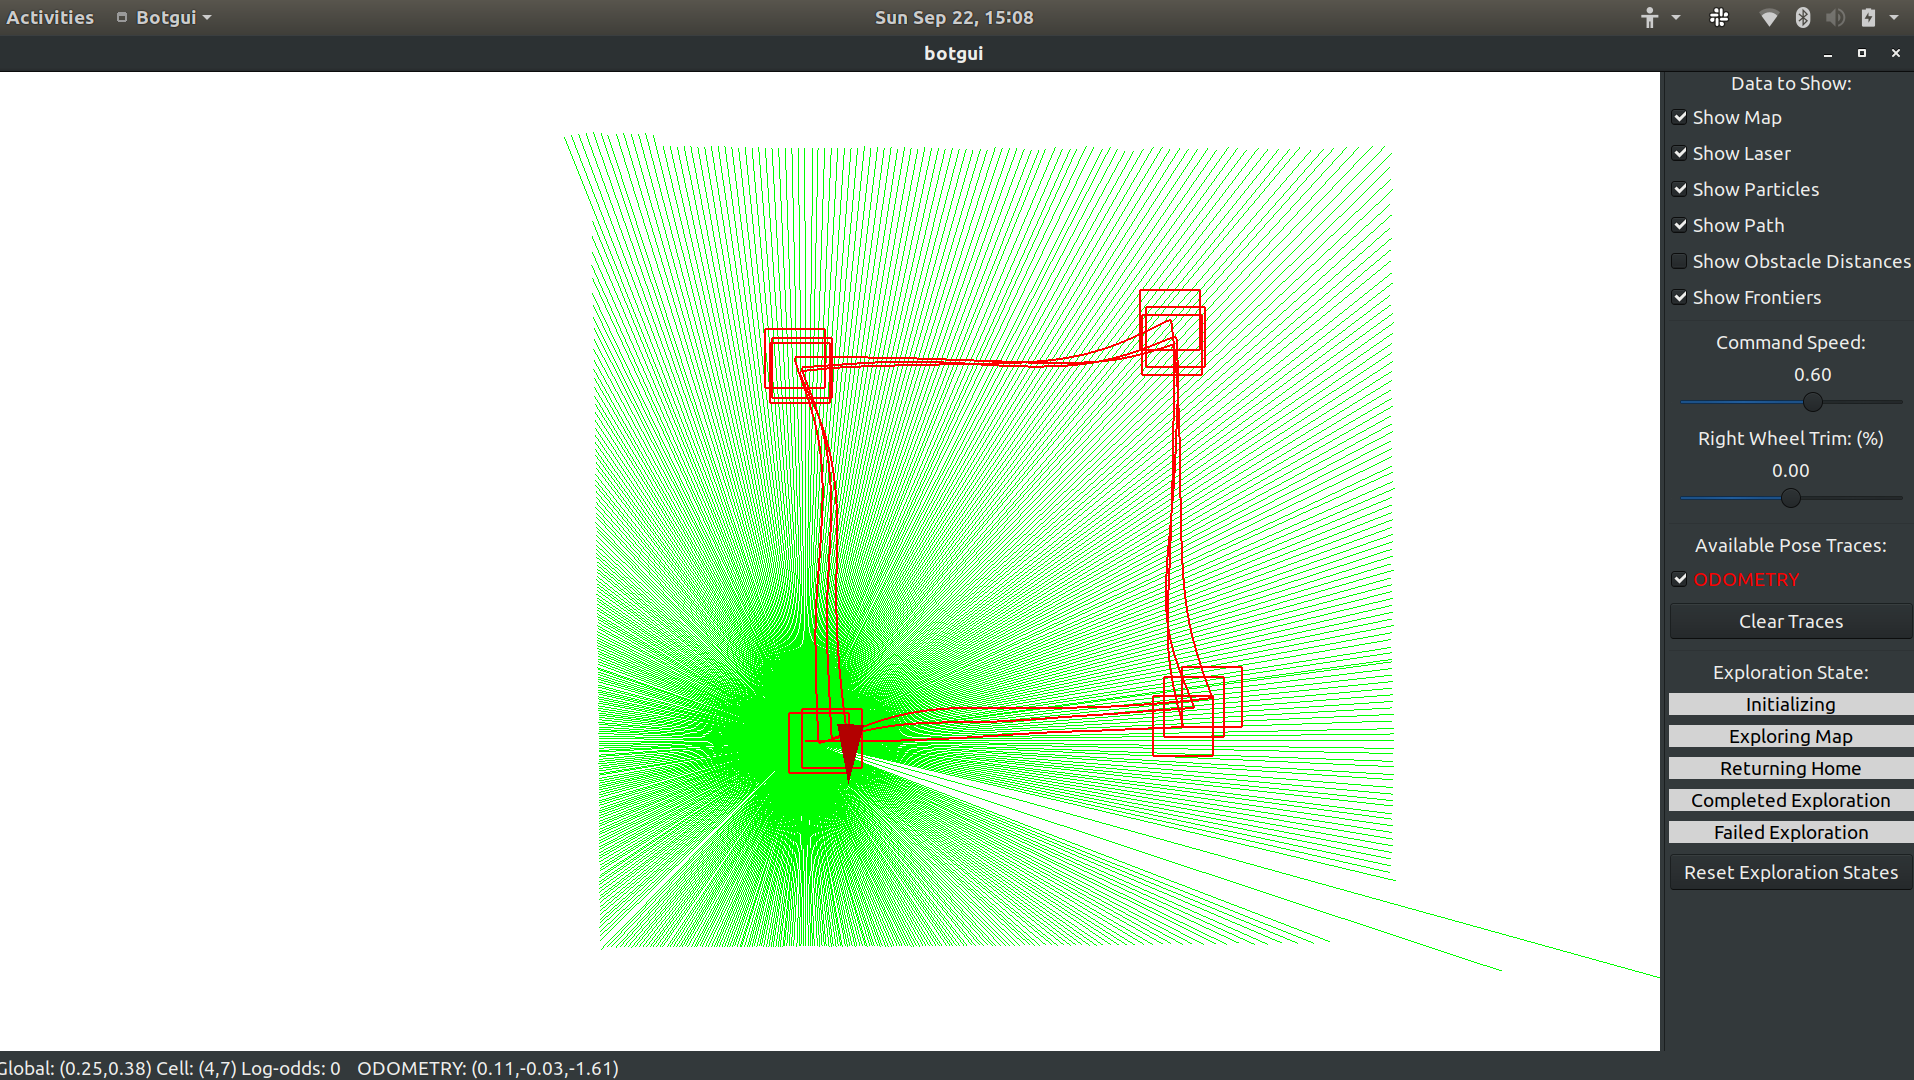
\includegraphics[width=\linewidth]{lidar_odometry_square.png}
\caption{Closed Loop Control with Laser Scans, visualized using odometry.}
\label{fig:task6}
\end{figure}
As you can see in figure 3, the odometry drifts gradually after running loops over loops.

We also visualize the world frame pose using distance to the right wall and distance to the front wall. The comparison between visualization using odometry and visualization using world frame pose of the same experiment is shown below.

\begin{figure}[H]
\centering
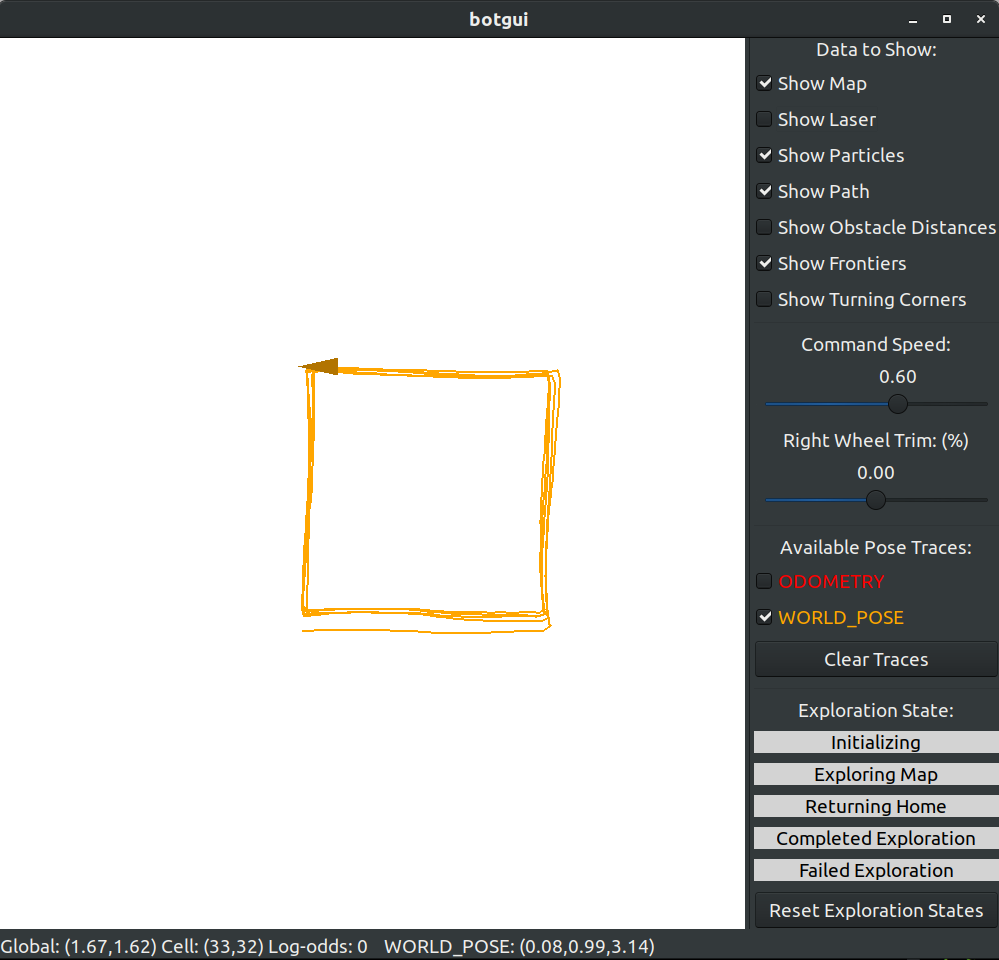
\includegraphics[width=\linewidth]{lidar_wf_pose.png}
\caption{Closed Loop Control with Laser Scans, visualized using world frame pose.}
\label{fig:task6}
\end{figure}

\begin{figure}[H]
\centering
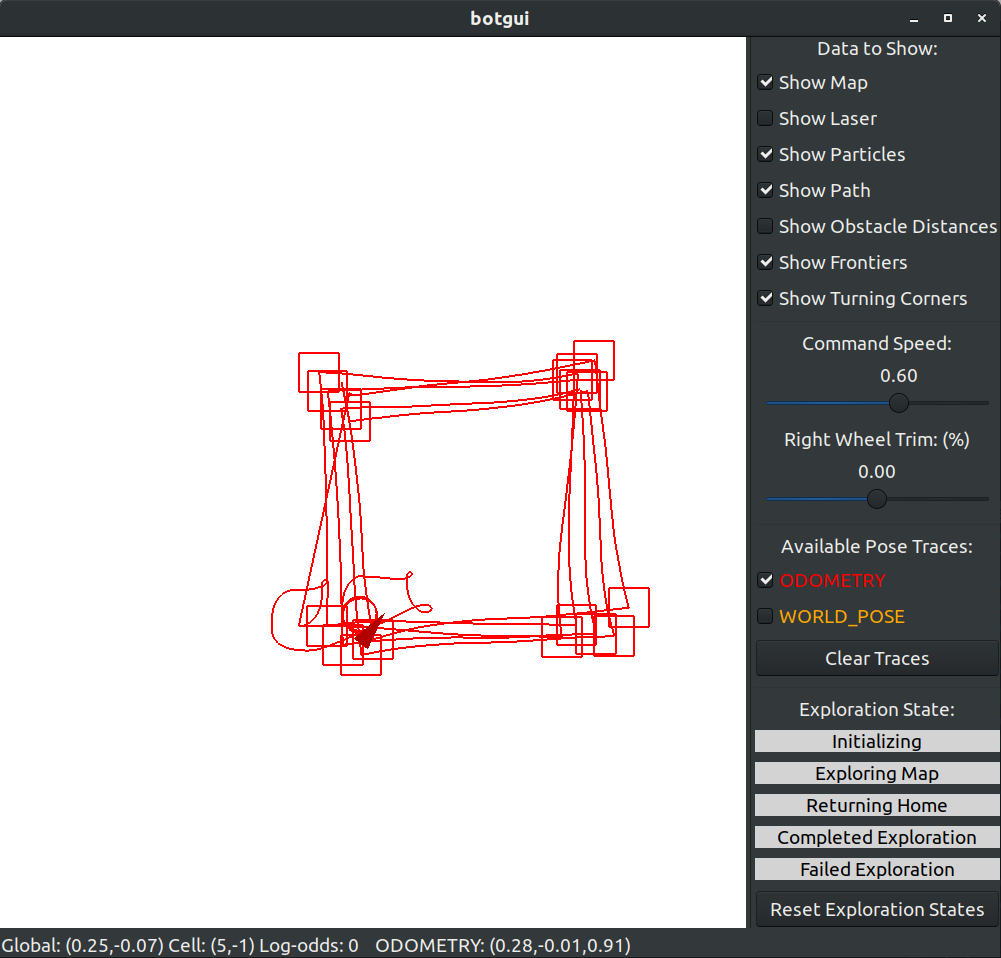
\includegraphics[width=\linewidth]{lidar_wf_with_turning_corner.png}
\caption{Closed Loop Control with Laser Scans, visualized using odometry.}
\label{fig:task6}
\end{figure}

As the robot runs, the odometry gradually drifts. But the world frame pose stays stable since we are using world frame pose to correct the trajectory of the robot.


\newpage
% \subsection{Certification}
\twocolumn[{%
\renewcommand\twocolumn[1][]{#1}%
\maketitle
\begin{center}
    \centering
    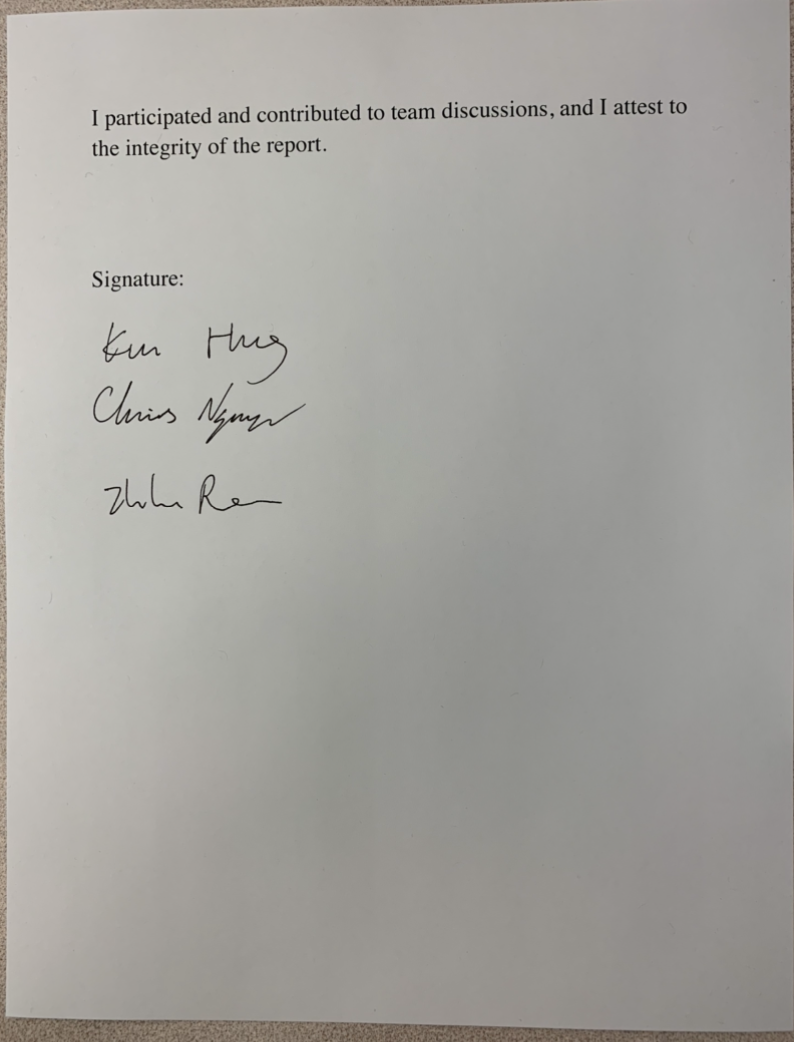
\includegraphics[width=.6\textwidth]{IMG_4687.PNG}
\end{center}%
}]


\clearpage
%%%%%%%%%%%%%%%%%%%%%%%%%%%%%%%%%%%%%%APPENDIX%%%%%%%%%%%%
\begin{appendices}
\onecolumn
\end{appendices}

\end{document}
